\documentclass[11pt]{article}
\usepackage{amsfonts,longtable}
\usepackage{amsmath}
\usepackage{amssymb}
\usepackage{amsthm}
\usepackage{esint}
\usepackage{mathdesign}
\usepackage{graphicx}
\usepackage{float}
\usepackage{bm}
\usepackage{cmap}
\usepackage[unicode]{hyperref}
\usepackage{epstopdf}
\usepackage[export]{adjustbox}
\usepackage[T2A]{fontenc}
\usepackage[utf8]{inputenc}
\usepackage[russian]{babel}
\usepackage{listings}
\usepackage{indentfirst}
\usepackage{changepage}
\usepackage{xcolor}
\usepackage{tikz}
\usepackage{pdfpages}
\usepackage{epsfig}
\usepackage[14pt]{extsizes} % для того чтобы задать нестандартный 14-ый размер шрифта
\usetikzlibrary{automata,positioning}

\definecolor{backcolour}{rgb}{0.95,0.95,0.92}
 
%Стиль для листинга
\lstdefinestyle{mystyle}{
    backgroundcolor=\color{backcolour},   
    commentstyle=\color{gray},
    keywordstyle=\color{magenta},
    numberstyle=\tiny\color{gray},
    stringstyle=\color{purple},
    basicstyle=\footnotesize,
    breakatwhitespace=false,         
    breaklines=true,                 
    captionpos=t,                    
    keepspaces=true,                 
    numbers=left,                    
    numbersep=5pt,                  
    showspaces=false,                
    showstringspaces=false,
    showtabs=false,                  
    tabsize=2
}

\graphicspath{ {img/} }
\textwidth=16cm
\oddsidemargin=1cm
\textheight=21cm
\topmargin=-1cm
\setlength\parindent{0pt}
\setcounter{MaxMatrixCols}{20}
\lstset{style=mystyle}
\parindent=1cm


\begin{document}

\begin{figure}[H]
	\begin{center}
		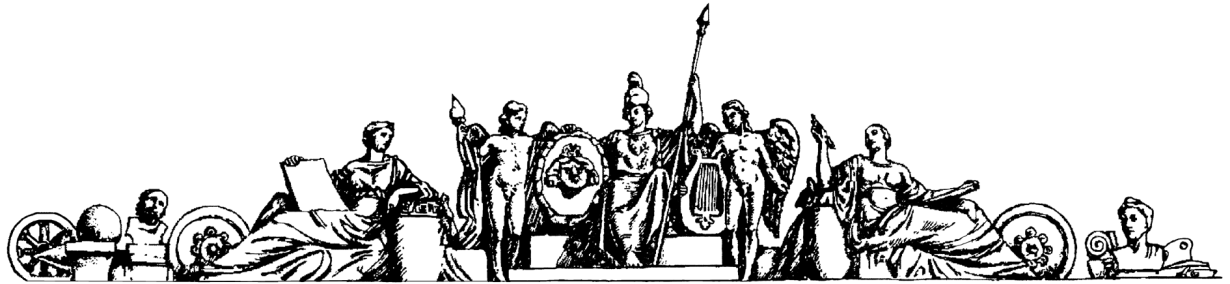
\includegraphics[width=5.59in,height=1.3in]{./img/titul.png}
	\end{center}
\end{figure}


%%%%%%%%%%%%%%%%%%%% Figure/Image No: 1 Ends here %%%%%%%%%%%%%%%%%%%%

\begin{center}
{\fontsize{14pt}{16.8pt}\selectfont Министерство Образования Российской Федерации\par}
\end{center}\par

\begin{center}
{\fontsize{14pt}{16.8pt}\selectfont Московский государственный технический университет имени Н.Э. Баумана\par}
\end{center}\par


\vskip 1cm
\begin{center}
{\fontsize{14pt}{16.8pt}\selectfont Факультет «Робототехника и комплексная автоматизация»\par}
\end{center}\par

\begin{center}
{\fontsize{14pt}{16.8pt}\selectfont Кафедра РК6 «Системы автоматизированного проектирования»\par}
\end{center}\par


\vspace{\baselineskip}

\vspace{\baselineskip}
\begin{center}
{\fontsize{14pt}{16.8pt}\selectfont Отчет по домашнему заданию \par}
\end{center}\par

\begin{center}
{\fontsize{14pt}{16.8pt}\selectfont по курсу "Аналитические модели и имитационное \\
моделирование на системном уровне" \par}
\end{center}\par

\vspace{\baselineskip}
\begin{flushright}
	Студент: \par \underline{Голубицкий С. Р.} \\ 
	Преподаватель:\par \underline{Берчун Ю. В.}
\end{flushright}



\vfill

\begin{center}
{\fontsize{14pt}{16.8pt}\selectfont Москва \the\year\par}
\end{center}\par

\newpage

\newpage
\section*{Задание 1}

\underline{Исходные данные:}
\begin{table}[h!]
    \begin{tabular} {|l|l|l|}
        \hline
        \textbf{Tc} & \textbf{Ts} & \textbf{Tw} \\ \hline
        28 & 231 &  529 \\ \hline
    \end{tabular}
\end{table}

Tc - среднее время между звонками клиентов

Ts - среднее время обслуживания

Tw - среднее время между звонками клиентов

\subsection*{Задание 1.1}

\underline{Условие:} Все потоки случайных событий считать пуассоновскими. Если все операторы заняты, звонок теряется. Рассчитать минимальное число операторов, при котором доля отказов не превышает 25\%, 10\%, 5\%, 1\%.
Построить график вероятности отказа от числа операторов. Построить график, иллюстрирующий коэффициент загрузки операторов в зависимости от их числа.
\\

\underline{Решение:}

Вероятность того, что ни один из операторов не будет занят, рассчитывается по формуле 1:

\begin{equation}
    P_0 = \frac{1}{\sum_{i=0}^N \frac{\lambda^i}{i! \mu^i}}
\end{equation}

, где

$P_0$ - вероятность того, что ни один из операторов не будет занят, 

$N$ - количесво операторов,

$\lambda$ - интенсивность поступления заявок, 

$\mu$ - интенсивность обработки заявок.
\\

Для расчета вероятности отказа воспользуемся формулой:

\begin{equation}
    P_{den} = \frac{\lambda^i}{i! \mu^i}P_0
\end{equation}

, где $P_den$ - вероятность отказа системы.
\\


Для расчета среднего количества занятых операторов используем формулу: 
\begin{equation}
    \overline{N} = \sum_{i=0}^N i P_i
\end{equation},
где \\ $\overline{N}$ - среднее количесво занятых операторов в системе\\
$P_i$ - вероятность отказа $i$-го оператора. 

Коэффицент загрузки операторов считается по форумуле 
$k = \frac{\overline{N}}{N}$, где $N$ - текущее число операторов.

\begin{figure}[h!]
    \centering
    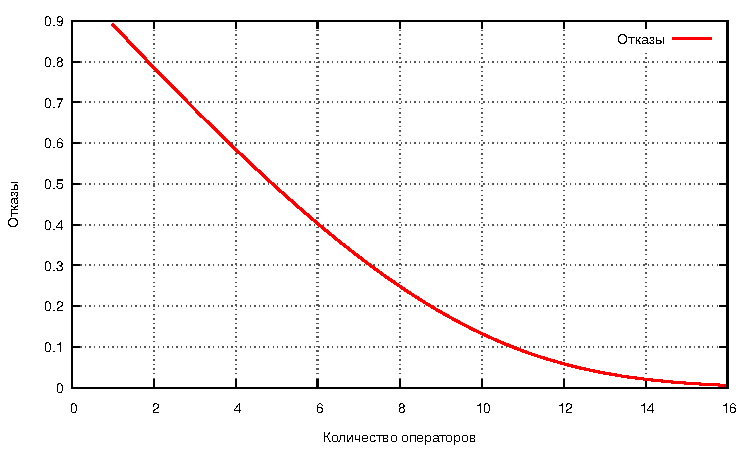
\includegraphics[width=0.7\textwidth]{z1.1/refuses.pdf}
    \caption{Зависимость отказов системы от количества операторов.}
\end{figure}

\begin{figure}[h!]
    \centering
    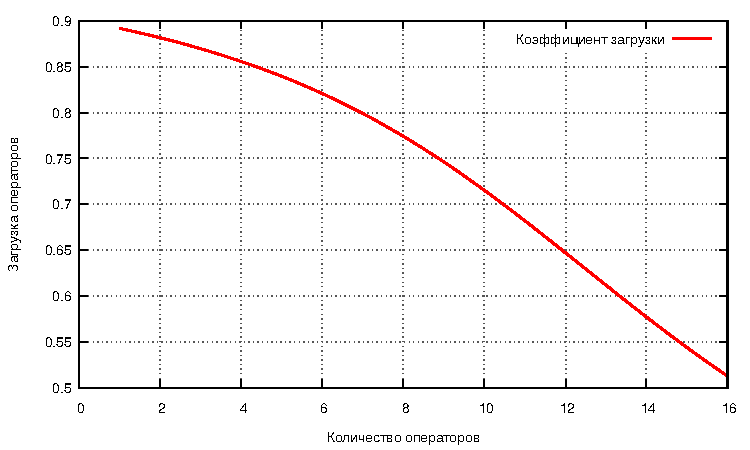
\includegraphics[width=0.7\textwidth]{z1.1/koeffzagrop.pdf}
    \caption{Зависимость отказов системы от количества операторов.}
\end{figure}
\subsection*{Задание 1.2}

\underline{Условие:}  Все потоки случайных событий считать пуассоновскими. Если все операторы заняты, звонок теряется. Построить график изменения доли отказов при замене каналов обслуживания местами в очереди (начиная с числа операторов, соответствующего 1\% отказов в системе без очереди). Построить график, иллюстрирующий коэффициент загрузки операторов. Построить график математического ожидания длины очереди. Построить график, иллюстрирующий коэффициент занятости мест в очереди. Построить график математического ожидания времени пребывания клиентов в очереди. 
\\

Решение:
Из задачи 1.1 известно, что при количестве операторов  N = 16 вероятность отказа системы составляет 0.6 \%. Для расчета вероятности, при которой операторы не будут заняты.
Тогда вероятность того, что операторы не заняты вычисляется по формуле:

\begin{equation}
    P_{0} = \frac{1}{\sum_{i=0}^{N} \frac{\lambda^i}{i! \mu^i}+\frac{\lambda^N}{N! \mu^N} \sum_{k=1}^{M}{(\frac{\lambda}{N \mu})^k}}
\end{equation}
, где M - количество мест в очереди.

Для расчета вероятности отказа системы можно воспользоваться формулой:

\begin{equation}
    P_{den} = \frac{\lambda^N}{N! \mu^N} (\frac{\lambda}{N \mu})^M P_0
\end{equation}

Расчет среднего количества занятых операторов ведется по формуле:

\begin{equation}
    \overline{N} = \sum_{i=0}^{N} i P_i + \sum_{k=1}^{M} N P_k
    \label{Naver}
\end{equation}

Матожидание длины очереди ведется по формуле:
\begin{equation}
    \overline{Q} = \sum_{k=1}^{M} k P_k
    \label{}
\end{equation}, 
где $\overline{Q}$ - матожидание длины очереди. Коэффицент занятости мест в очереди вычисляется по формуле:
$k = \frac{\overline{Q}}{Q}$, где k - коэффициент занятости мест в очереди.

Среднее время ожидания в очереди вычисляется по формуле: \\$\Delta \overline{t} =  \frac{\overline{Q}}{\lambda}$.  


\begin{figure}[H]
	\begin{center}
        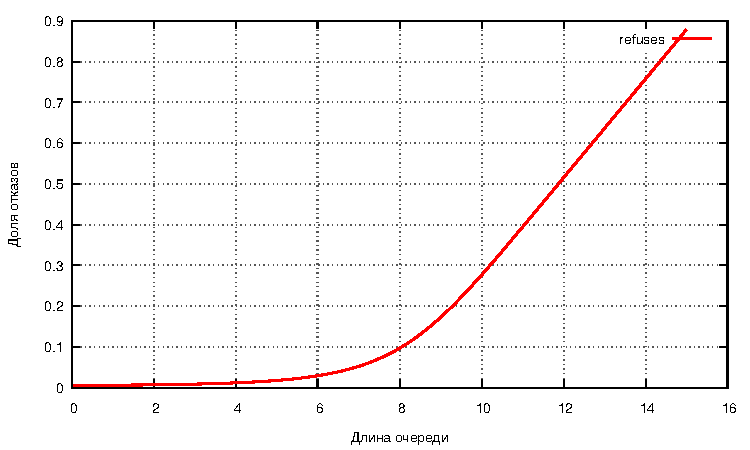
\includegraphics{/z1.2/qref.pdf}
        \caption{Зависимость вероятности отказа системы от мест в очереди}
	\end{center}
\end{figure}

\begin{figure}[H]
	\begin{center}
        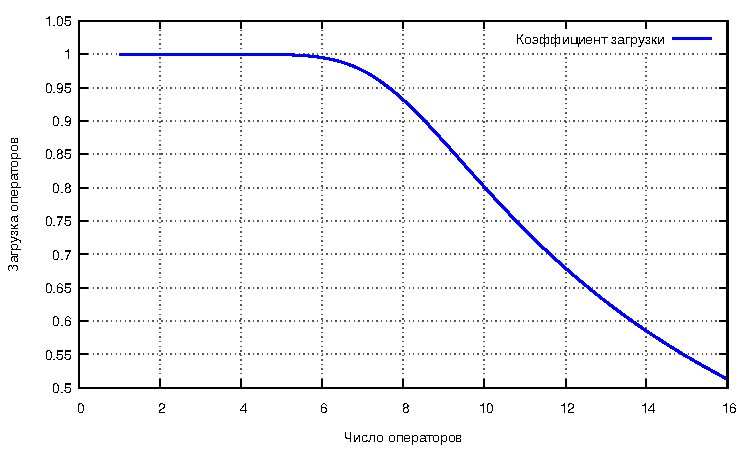
\includegraphics{/z1.2/kcpref.pdf}
        \caption{Зависимость коэффициента загрузки операторов от их общего количества}
	\end{center}
\end{figure}

\begin{figure}[H]
	\begin{center}
        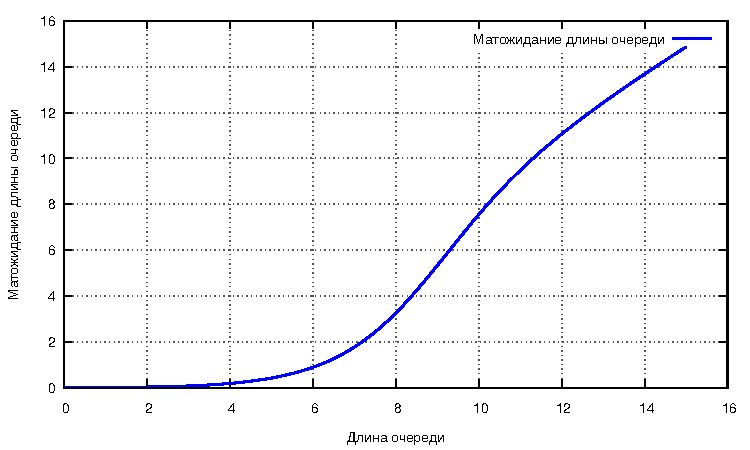
\includegraphics{/z1.2/matozh.pdf}
        \caption{Зависимость математического ожидания длины очереди от мест в очереди}
	\end{center}
\end{figure}

\begin{figure}[H]
	\begin{center}
        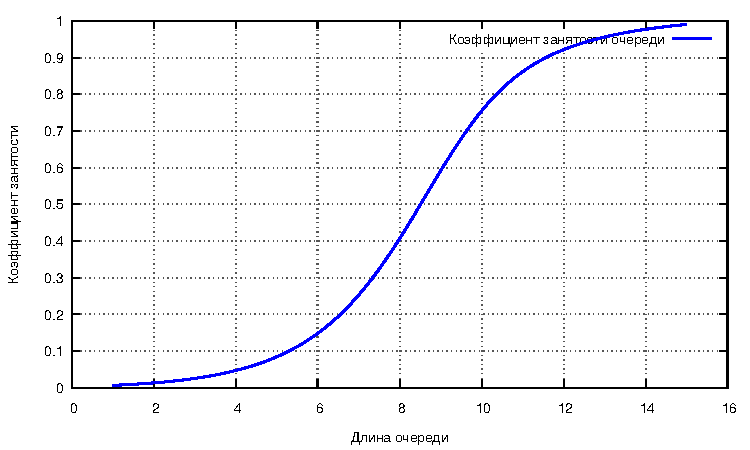
\includegraphics{/z1.2/queucoeff.pdf}
        \caption{Зависимость коэффициента занятости мест в очереди от длины очереди}
	\end{center}
\end{figure}

\begin{figure}[H]
	\begin{center}
        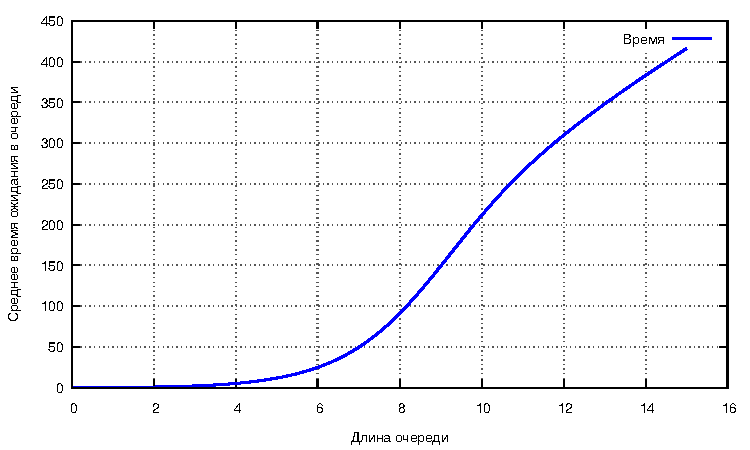
\includegraphics{/z1.2/qwtime.pdf}
        \caption{Зависимость математического ожидания времени ожидания в очереди от мест в очереди}
	\end{center}
\end{figure}
\subsection*{Задание 1.3}

\underline{Условие:} Все потоки случайных событий считать пуассоновскими. Если все операторы заняты, звонок теряется. Рассмотреть систему без ограничений на длину очереди. Построить график математического ожидания длины очереди в зависимости от числа операторов (вплоть до числа каналов, соответствующего 1$\%$  отказов в системе без очереди). Построить график, иллюстрирующий коэффициент загрузки операторов. Построить график математического ожидания времени пребывания клиентов в очереди.\par

\underline{Решение:}\par

Для расчета вероятности, при которой операторы не будут заняты, можно воспользоваться формулой 11:\par


\begin{equation} \label{P0}
    P_{0}=\frac{1}{ \sum _{i=0}^{N}\frac{ \lambda ^{i}}{i! \cdot  \mu ^{i}}+\frac{ \lambda ^{N}}{N! \cdot  \mu ^{N}} \cdot  \sum _{k=1}^{\infty} \left( \frac{ \lambda }{N \cdot  \mu } \right) ^{k}} 
\end{equation} \par

Практический интерес будут представлять такие варианты системы, при которых сумма  \(  \sum _{k=1}^{\infty} \left( \frac{ \lambda }{N \cdot  \mu } \right) ^{k}  \) будет сходящейся. Для того, чтобы данная сумма сходилась необходимо, чтобы член  \( \frac{ \lambda }{N \cdot  \mu }  \) был\ меньше единицы. Исходя из начальных условий практический смысл представляет  рассмотрение систем, где  \( N \geq 9. \)  При таких условиях выражение \ref{P0} можно преобразовать к следующему виду:\par

\begin{equation}
 P_{0}=\frac{1}{ \sum _{i=0}^{N}\frac{ \lambda ^{i}}{i! \cdot  \mu ^{i}}+\frac{ \lambda ^{N}}{N! \cdot  \mu ^{N}} \cdot \frac{ \lambda }{N \cdot  \mu - \lambda }}
\end{equation} \par

Для расчета математического ожидания длины очереди можно воспользeмся формулой:\par

  \begin{equation} \overline{Q}=\frac{ \lambda ^{N}}{N! \cdot  \mu ^{N}} \cdot P_{0} \cdot \frac{a}{ \left( 1-a \right) ^{2}}     \end{equation} \par

где  \( a= \frac{ \lambda }{N \cdot  \mu } \) .\par

Для расчета среднего количества занятых операторов можно воспользоваться\\
формулой:\par

\begin{equation}
 \overline{N}=P_{0} \cdot  \left(  \sum _{i=1}^{N}\frac{ \lambda ^{i}}{ \left( i-1 \right) ! \cdot  \mu ^{i}}+ \frac{ \lambda ^{N}}{ \left( N-1 \right) ! \cdot  \mu ^{N}} \cdot \frac{ \lambda }{N \cdot  \mu - \lambda } \right) 
\end{equation} \par

\begin{figure}[H]
	\begin{center}
        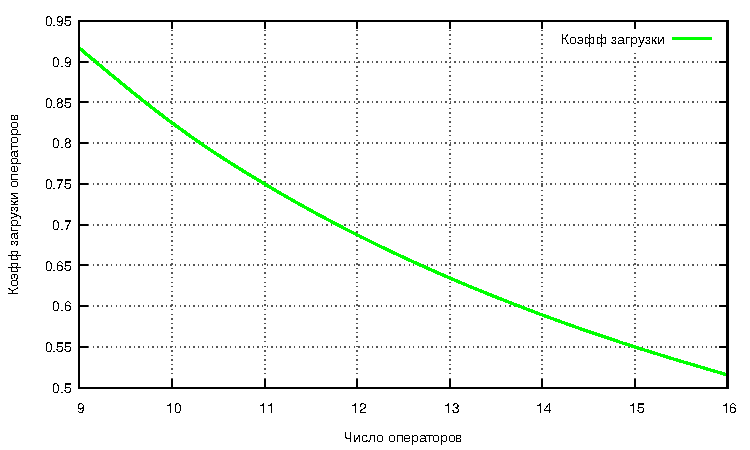
\includegraphics{/z1.3/ninf.pdf}
        \caption{Зависимость коэффициента загрузки операторов от их общего количества}
	\end{center}
\end{figure}


\begin{figure}[H]
	\begin{center}
        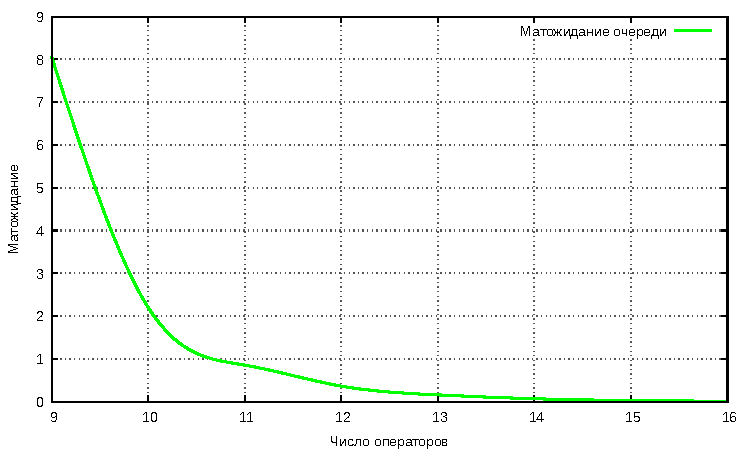
\includegraphics{/z1.3/qinf.pdf}
        \caption{Зависимость математического ожидания длины очереди от количества операторов}
	\end{center}
\end{figure}

\begin{figure}[H]
	\begin{center}
        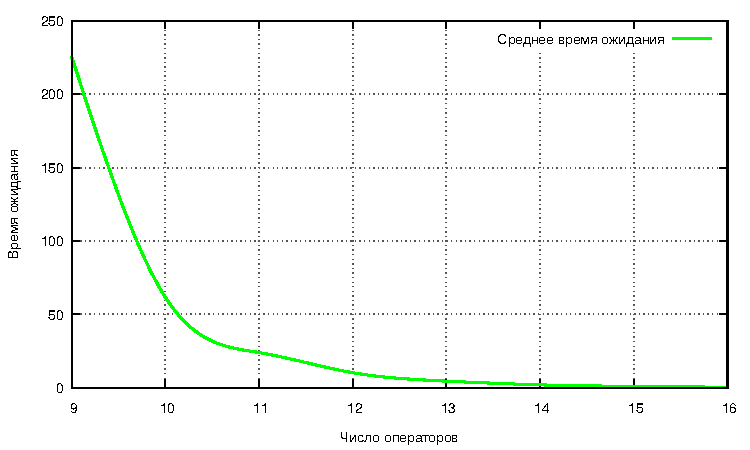
\includegraphics{/z1.3/tinf.pdf}
        \caption{Зависимость математического ожидания времени ожидания в очереди от количества операторов}
	\end{center}
\end{figure}


\subsection*{Задание 1.4}


\underline{Условие:} Все потоки случайных событий считать пуассоновскими. Если все операторы заняты, звонок теряется. Рассмотреть систему без ограничений на длину очереди, учитывающей фактор ухода клиентов из очереди (среднее приемлемое время ожидания – Tw секунд). Построить график средней длины очереди в зависимости от числа операторов (вплоть до числа каналов, соответствующего 1$\%$  отказов в системе без очереди). Построить график, иллюстрирующий коэффициент загрузки операторов. Построить график математического ожидания времени пребывания клиентов в очереди.\par

\underline{Решение:}\par

Для расчета вероятности, при которой операторы не будут заняты, можно воспользоваться формулой 15:\par

\begin{equation}
     P_{0}=\frac{1}{ \sum _{i=0}^{N}\frac{ \lambda ^{i}}{i! \cdot  \mu ^{i}}+\frac{ \lambda ^{N}}{N! \cdot  \mu ^{N}} \cdot  \sum _{k=1}^{\infty}\frac{ \lambda ^{k}}{ \prod_{j=1}^{k} \left( N \cdot  \mu +j \cdot  \upsilon  \right) }}  
\end{equation} \par

где  \(  \upsilon -  \) интенсивность выхода из очереди.\par

Для расчета математического ожидания длины очереди можно воспользуемся формулой:

\begin{equation}
    \overline{Q}= \sum _{k=1}^{\infty}\frac{k \cdot  \lambda ^{k}}{ \prod_{j=1}^{k} \left( N \cdot  \mu +j \cdot  \upsilon  \right) } \cdot \frac{ \lambda ^{N}}{N! \cdot  \mu ^{N}} \cdot P_{0}
\end{equation} \par

Для расчета среднего количества занятых операторов можно воспользуемся формулой:

 \begin{multline} 
    \overline{N} = \\ P_{0}  \cdot  \left(  \sum _{i=1}^{N}\frac{ \lambda ^{i}}{ \left( i-1 \right) ! \cdot  \mu ^{i}}+ \frac{ \lambda ^{N}}{ \left( N-1 \right) ! \cdot  \mu ^{N}} \cdot   \sum _{k=1}^{\infty}\frac{ \lambda ^{k}}{ \prod_{j=1}^{k} \left( N \cdot  \mu +j \cdot  \upsilon  \right) } \right) 
\end{multline} \par

\begin{figure}[H]
	\begin{center}
        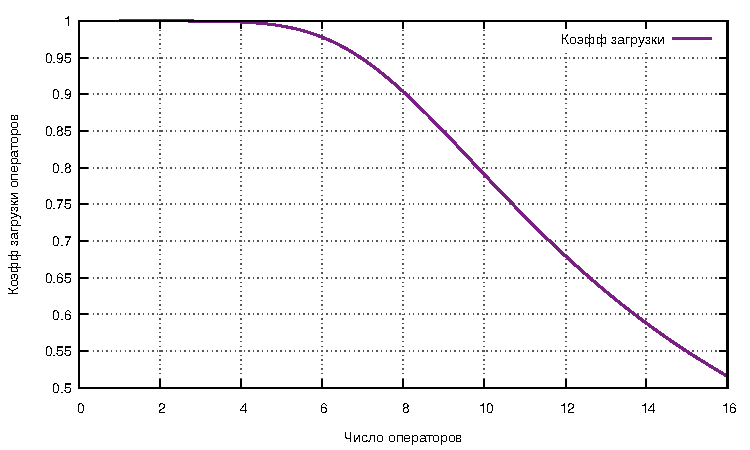
\includegraphics{/z1.4/ninftime.pdf}
        \caption{Зависимость коэффициента загрузки операторов от их общего количества}
	\end{center}
\end{figure}


\begin{figure}[H]
	\begin{center}
        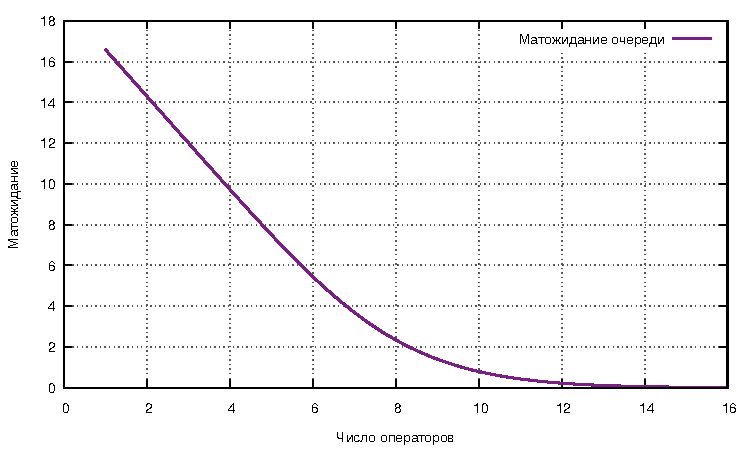
\includegraphics{/z1.4/qinftime.pdf}
        \caption{Зависимость математического ожидания длины очереди от количества операторов}
	\end{center}
\end{figure}


\begin{figure}[H]
	\begin{center}
        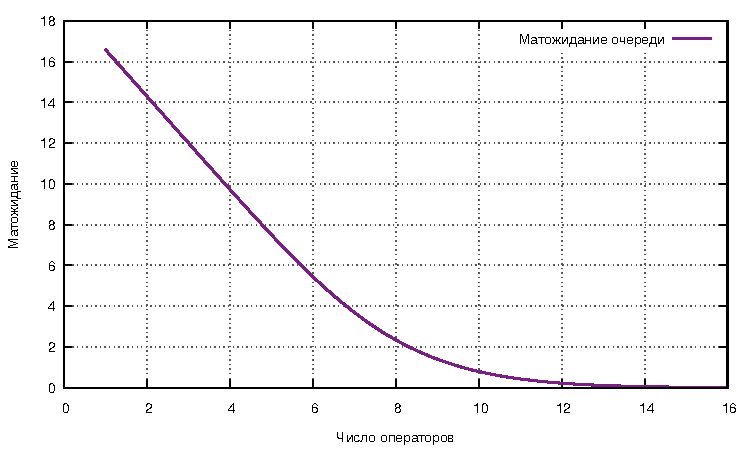
\includegraphics{/z1.4/qinftime.pdf}
        \caption{Зависимость математического ожидания времени ожидания в очереди от количества операторов}
	\end{center}
\end{figure}

\section*{Задание 2}

\underline{Исходные данные:}
\begin{table}[h!]
    \begin{tabular} {|l|l|l|}
        \hline
        \textbf{Tc} & \textbf{Ts} & \textbf{n} \\ \hline
        330 & 11 &  40 \\ \hline
    \end{tabular}
\end{table}

Tc - среднее время между наладками

Ts - среднее время наладки

n - число станков

\subsection*{Задача 2.1}

\underline{Условие:} имеется участок с N станками. Среднее время между наладками составляет Tc минут, среднее время наладки – Ts минут. Все потоки случайных событий считать пуассоновскими. Построить график зависимости числа простаивающих станков от числа наладчиков. Построить график зависимости числа станков, ожидающих обслуживания, от числа наладчиков. Построить график зависимости среднего числа занятых наладчиков от их числа. Построить график зависимости коэффициента занятости наладчиков от их числа.\par

\underline{Решение:}\par

Для расчета вероятности, при которой все станки будут налажены, можно воспользоваться формулой:

\begin{equation}
    P_{0}=\frac{1}{1+ \sum _{i=1}^{M}\frac{ \prod_{j=1}^{i} \left( N-j+1 \right)  \cdot  \lambda ^{i}}{i! \cdot  \mu ^{i}}+ \sum _{k=M+1}^{N}\frac{ \prod_{j=1}^{k} \left( N-j+1 \right) }{M! \cdot M^{k-M}} \cdot  \left( \frac{ \lambda }{ \mu } \right) ^{k}}
\end{equation} 

где  \( P_{0}-  \) вероятность, при которой все станки будут налажены;\par

 \( M-  \) количество наладчиков;\par

 \( N-  \) количество станков;\par

 \(  \lambda -  \) интенсивность поломки станков;\par

 \(  \mu -  \) интенсивность наладки станков.\par

Для расчета числа ожидающих наладки станков можно воспользоваться формулой 19:\par

\begin{equation} 
    \overline{N}_{ожид.}=P_{0} \cdot  \sum _{k=M+1,~ i=1}^{N, N-M}\frac{i \cdot  \prod_{j=1}^{k} \left( N-j+1 \right) }{M! \cdot M^{k-M}} \cdot  \left( \frac{ \lambda }{ \mu } \right) ^{k} 
\end{equation} \par

где  \( \overline{N}_{ожид.}-  \) среднее количество ожидающих наладки станков.\par

Для расчета числа простаивающих станков можно воспользоваться формулой 20:\par

\begin{equation}
    \overline{N}_{прост.}=P_{0} \cdot  \sum _{i=1}^{M}\frac{i \cdot  \prod_{j=1}^{i} \left( N-j+1 \right)  \cdot  \lambda ^{i}}{i! \cdot  \mu ^{i}} + P_{0} \cdot  \sum _{k=M+1}^{N}\frac{k \cdot  \prod_{j=1}^{k} \left( N-j+1 \right) }{M! \cdot M^{k-M}} \cdot  \left( \frac{ \lambda }{ \mu } \right) ^{k}
\end{equation} \par

где  \( \overline{N}_{прост.}-  \) среднее количество простаивающих станков.\par

Для расчета среднего числа занятых наладчиков можно воспользоваться формулой 21:\par

\begin{equation}
    \overline{M}_{зан.}=P_{0} \cdot  \sum _{i=1}^{M}\frac{i \cdot  \prod_{j=1}^{i} \left( N-j+1 \right)  \cdot  \lambda ^{i}}{i! \cdot  \mu ^{i}} + P_{0} \cdot M \cdot  \sum _{k=M+1}^{N}\frac{ \prod_{j=1}^{k} \left( N-j+1 \right) }{M! \cdot M^{k-M}} \cdot  \left( \frac{ \lambda }{ \mu } \right) ^{k}
\end{equation} \par

где  \( \overline{M}_{зан.}-  \) среднее количество занятых наладчиков.\par

Для расчета коэффициента занятости наладчиков от их числа можно воспользоваться формулой 22:\par

 \begin{equation}
    k_{M}=\frac{\overline{M}_{зан.}}{M} 
\end{equation} \par

 \( k_{M}-  \) коэффициент занятости наладчиков.\par


\begin{figure}[H]
	\begin{center}
        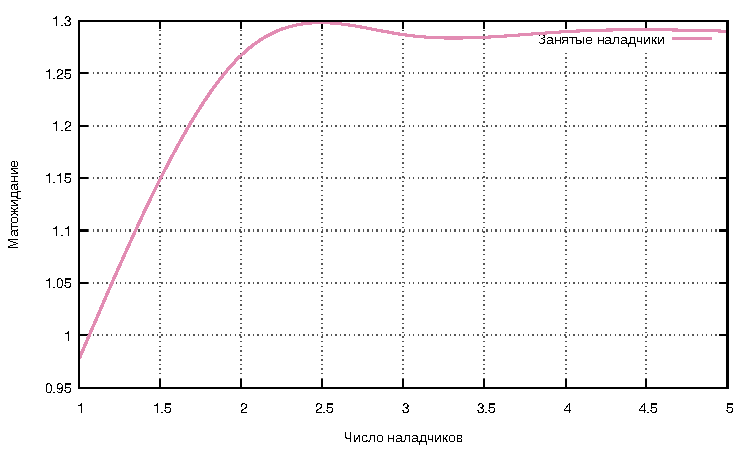
\includegraphics{/z2/mz.pdf}
        \caption{Зависимость математического ожидания ожидающих наладки станков от количества наладчиков}
	\end{center}
\end{figure}

\begin{figure}[H]
	\begin{center}
        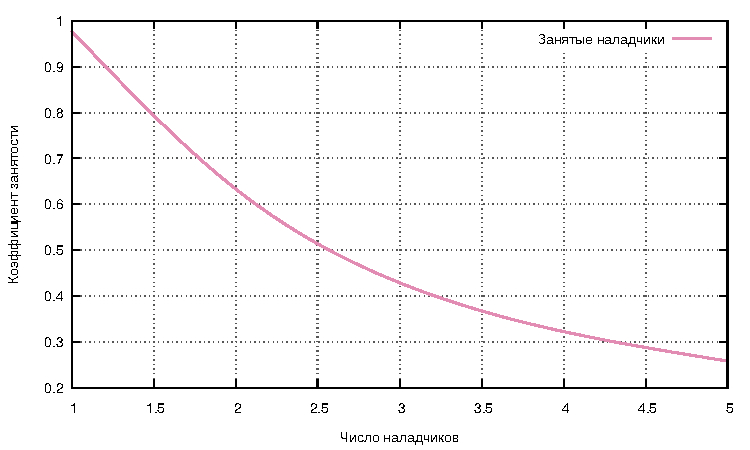
\includegraphics{/z2/mzdn.pdf}
        \caption{Зависимость математического ожидания простаивающих станков от количества наладчиков}
	\end{center}
\end{figure}

\begin{figure}[H]
	\begin{center}
        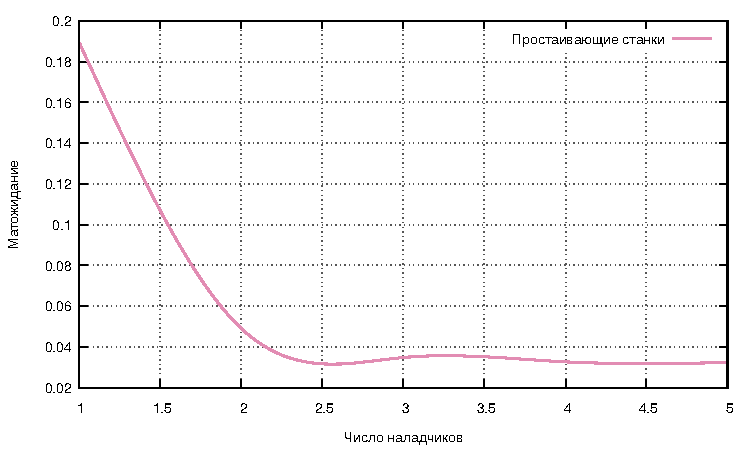
\includegraphics{/z2/nprost.pdf}
        \caption{Зависимость математического ожидания простаивающих станков от количества наладчиков}
	\end{center}
\end{figure}

\begin{figure}[H]
	\begin{center}
        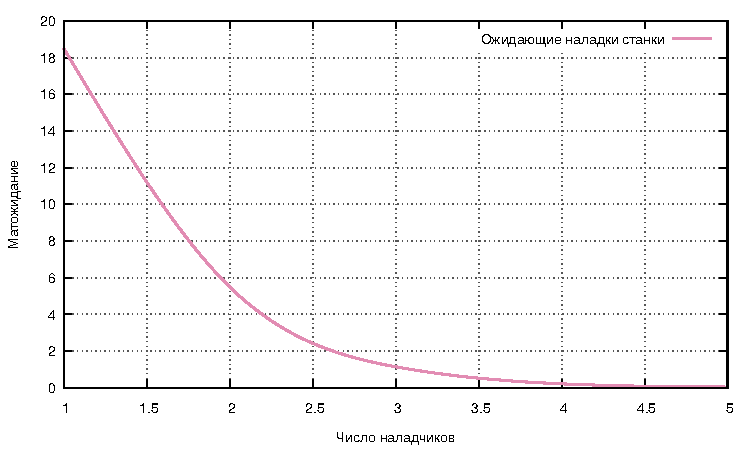
\includegraphics{/z2/nozh.pdf}
        \caption{Зависимость коэффициента занятости наладчиков от их числа}
	\end{center}
\end{figure}

\end{document}


